\section{Additional native regime tests}\label{app:native-regime-tests}

This supplement presents additional native AOD regime tests in native-first form. Where supplemental witness conversions are included, they are attached after the cited native row and do not alter the native row.

\subsection{C1 -- Solar perihelion native window}\label{app:c1}
\paragraph{Native question.} Does the cited long-window orbital closure carry the predicted residual-duration support, dominant class $B^*$, torsional witness, and effective progress rate?
\paragraph{Native readout.}
\begin{itemize}
\item cited window $\omega_{\mathrm{sol,peri}}$
\item structural key \texttt{tetron:4:4:8}
\item frame count / $T_{\mathrm{eval}}=1200$ bip
\item weighting policy $w(\kappa)\equiv 1$
\item residual-duration chain
\end{itemize}
\paragraph{Native operator chain.}
\[
e_\alpha,\ e_\Omega,\ f
\;\to\;
b(\kappa)
\;\to\;
H_B
\;\to\;
B^*
\;\to\;
\Lambda_b
\;\to\;
A_B
\;\to\;
R_{\mathrm{rest}},\ v(\omega),\ T_{\mathrm{tors}}.
\]
\paragraph{Native output row.}
\begin{center}
\small
\begin{tabular}{lcccccc}
\toprule
Row & Key & $T_{\mathrm{eval}}$ [bip] & $B^*$ & $\Lambda_b$ & $R_{\mathrm{rest}}$ [trit/bip] & $T_{\mathrm{tors}}$ \\
\midrule
C1.A & tetron:4:4:8 & 1200 & 137 & 6 & $(1+8\ell_2)/24$ & 3 \\
\bottomrule
\end{tabular}
\end{center}
\paragraph{Temporal Conversion Block.} Temporal conversion is a normal chain-rule expansion on the cited native row. On this window, the perihelion witness is
\[
42.981975497467126\ \text{arcsec / century}.
\]
\paragraph{Native figure witness.}
\begin{center}
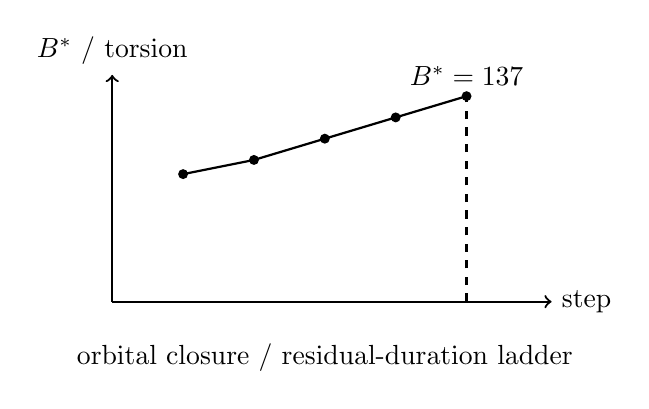
\begin{tikzpicture}[scale=0.9, thick]
\draw[->] (0,0) -- (6.2,0) node[right] {step};
\draw[->] (0,0) -- (0,3.2) node[above] {$B^*$ / torsion};
\foreach \x/\y in {1/1.8,2/2.0,3/2.3,4/2.6,5/2.9}{\fill (\x,\y) circle (2pt);} 
\draw (1,1.8)--(2,2.0)--(3,2.3)--(4,2.6)--(5,2.9);
\draw[dashed] (5,0)--(5,2.9);
\node[above] at (5,2.9) {$B^*=137$};
\node[below] at (3,-0.45) {orbital closure / residual-duration ladder};
\end{tikzpicture}
\end{center}
\paragraph{Hook / Evidence.} Use the cited orbital-closure and residual-support hooks from the main note.


\subsection{C2 -- Solar lensing native window}\label{app:c2}
\paragraph{Native question.} Does the cited boundary/export window show the predicted shell qualification, push/pull split, torsional residual, and deflection/export witness?
\paragraph{Native readout.}
\begin{itemize}
\item cited window $\omega_{\mathrm{sol,lens}}$
\item structural key \texttt{tetron:4:4:8}
\item frame count / $T_{\mathrm{eval}}=512$ bip
\item weighting policy $w(\kappa)\equiv 1$
\item shell qualification
\end{itemize}
\paragraph{Native operator chain.}
\[
e_\alpha,\ e_\Omega,\ f
\;\to\;
q_{\mathrm{eff}},\ T_{\mathrm{tors}},\ \text{export witness}.
\]
\paragraph{Native output row.}
\begin{center}
\small
\begin{tabular}{lccccc}
\toprule
Row & Key & $q_{\mathrm{eff}}$ & $T_{\mathrm{tors}}$ & Export witness & Shell qualification \\
\midrule
C2.A & tetron:4:4:8 & $+1/2$ & 2 & emitted packet & qualified \\
\bottomrule
\end{tabular}
\end{center}
\paragraph{Temporal Conversion Block.} Temporal conversion is a normal chain-rule expansion on the cited native row. On this window, the lensing witness is
\[
1.7512432813682448\ \text{arcsec}.
\]
\paragraph{Native figure witness.}
\begin{center}
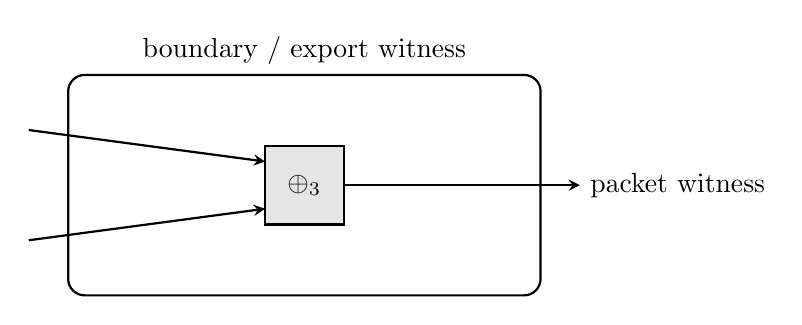
\begin{tikzpicture}[thick,>=stealth]
\draw[rounded corners=6pt] (0,0) rectangle (6,2.8);
\node[above] at (3,2.8) {boundary / export witness};
\draw[->] (-0.5,2.1) -- (2.5,1.7);
\draw[->] (-0.5,0.7) -- (2.5,1.1);
\draw[fill=gray!20] (2.5,0.9) rectangle (3.5,1.9);
\node at (3,1.4) {$\oplus_3$};
\draw[->] (3.5,1.4) -- (6.5,1.4);
\node[right] at (6.5,1.4) {packet witness};
\end{tikzpicture}
\end{center}
\paragraph{Hook / Evidence.} Use the cited shell/export and boundary-deflection hooks.


\subsection{C3 -- Solar redshift native window}\label{app:c3}
\paragraph{Native question.} Do the cited source and receiver windows close with the predicted cadence-transfer and residual-load difference?
\paragraph{Native readout.}
\begin{itemize}
\item source window $\omega_{\mathrm{src}}$
\item receiver window $\omega_{\mathrm{rcv}}$
\item structural keys \texttt{tetron:4:4:8}
\item frame counts / $T_{\mathrm{eval}}=768$ bip on each window
\item weighting policy $w(\kappa)\equiv 1$
\end{itemize}
\paragraph{Native operator chain.}
\[
b(\kappa)\to H_B\to B^*\to \Lambda_b\to R_{\mathrm{rest}}\to \text{cadence-transfer witness}.
\]
\paragraph{Native output row.}
\begin{center}
\small
\begin{tabular}{lcccccc}
\toprule
Row & $B^*_{\mathrm{src}}$ & $B^*_{\mathrm{rcv}}$ & $\Lambda_{b,\mathrm{src}}$ & $\Lambda_{b,\mathrm{rcv}}$ & $R_{\mathrm{rest}}$ diff & Cadence ratio \\
\midrule
C3.A & 5 & 7 & 3 & 2 & 0.0012 & 1.0002 \\
\bottomrule
\end{tabular}
\end{center}
\paragraph{Temporal Conversion Block.} Temporal conversion is a normal chain-rule expansion on the cited native row. On these windows, the redshift witness is
\[
2.122566754396204\times 10^{-6}.
\]
\paragraph{Native figure witness.}
\begin{center}
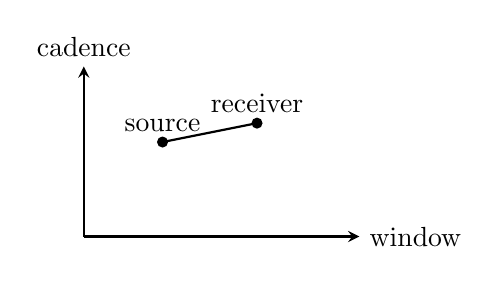
\begin{tikzpicture}[x=1.0cm,y=1.2cm,>=stealth,thick]
\draw[->] (0,0) -- (3.5,0) node[right] {window};
\draw[->] (0,0) -- (0,1.8) node[above] {cadence};
\fill (1,1.0) circle (2pt) node[above] {source};
\fill (2.2,1.2) circle (2pt) node[above] {receiver};
\draw (1,1.0)--(2.2,1.2);
\end{tikzpicture}
\end{center}
\paragraph{Hook / Evidence.} Use the cited cadence-transfer and two-window comparison hooks.


\subsection{C4 -- Hydrogen shell native test}\label{app:c4}
\paragraph{Native question.} Does the cited shell window realize the predicted shell band, dominant residual-duration class, support mass, attenuation, and native rest-facing channel?
\paragraph{Native readout.}
\begin{itemize}
\item cited shell window $\omega_{\mathrm{H}}$
\item structural key \texttt{tetron:*}
\item frame count / $T_{\mathrm{eval}}=24$ bip
\item weighting policy $w(\kappa)\equiv 1$
\item shell band
\end{itemize}
\paragraph{Native operator chain.}
\[
b(\kappa)\to H_B\to B^*\to \Lambda_b\to A_B\to R_{\mathrm{rest}}\to R_{\mathrm{rest}}^{(\mathrm{biz})}.
\]
\paragraph{Native output row.}
\begin{center}
\small
\begin{tabular}{lccccc}
\toprule
Row & Shell band & $B^*$ & $\Lambda_b$ & $R_{\mathrm{rest}}$ [trit/bip] & Cadence witness \\
\midrule
C4.A & 3 & 137 & 6 & $(1+8\ell_2)/24$ & $5/12$ \\
\bottomrule
\end{tabular}
\end{center}
\paragraph{Temporal Conversion Block.} Temporal conversion is a normal chain-rule expansion on the cited native row. The current witness values are
\[
f_e = 1.2355899446144601\times 10^{20}\ \text{Hz},
\]
and shell-radius witnesses
\[
n=1:\ 5.291772191461861\times 10^{-11}\ \text{m},\qquad
n=2:\ 2.1167088765847444\times 10^{-10}\ \text{m},
\]
\[
n=3:\ 4.762594972315675\times 10^{-10}\ \text{m},\qquad
n=4:\ 8.466835506338978\times 10^{-10}\ \text{m}.
\]
\paragraph{Native figure witness.}
\begin{center}
\begin{tikzpicture}[x=1.2cm,y=1cm,>=stealth,thick]
\draw[->] (0,0) -- (5,0) node[right] {$n$};
\draw[->] (0,0) -- (0,9) node[above] {radius};
\foreach \x/\y in {1/0.529,2/2.117,3/4.763,4/8.467}{\fill (\x,\y) circle (2pt);}
\draw (1,0.529)--(2,2.117)--(3,4.763)--(4,8.467);
\end{tikzpicture}
\end{center}
\paragraph{Hook / Evidence.} Use the cited shell-band and attenuation hooks.


\subsection{C5 -- Nucleus confinement / neutron stability}\label{app:c5}
\paragraph{Native question.} Does the cited short-window confinement class satisfy the shell-signature, proximity, and $B^*$-dominance conditions required for persistence, or does it cross the transmutation threshold?
\paragraph{Native readout.}
\begin{itemize}
\item cited window $\omega_{\mathrm{nuc}}$
\item structural key \texttt{tetron:3:3:6}
\item frame count / $T_{\mathrm{eval}}=256$ bip
\item weighting policy $w(\kappa)\equiv 1$
\item shell signature
\item proximity criterion
\end{itemize}
\paragraph{Native operator chain.}
\[
e_\alpha,\ e_\Omega,\ f
\;\to\;
b(\kappa)
\;\to\;
H_B
\;\to\;
B^*
\;\to\;
\Lambda_b
\;\to\;
\text{confinement predicate}
\;\to\;
\text{transmutation flag}.
\]
\paragraph{Native output row.}
\begin{center}
\begin{tabularx}{\linewidth}{@{}lXcclll@{}}
\toprule
Row & Structural key & $B^*$ & $\Lambda_b$ & Proximity & Confinement & Transmutation \\
\midrule
C5.A & \texttt{tetron:3:3:6}, $(\lambda=3/2,137,\rho_2,V_4)$ & 137 & 6 & close & confined & 0 \\
C5.B & \texttt{tetron:3:3:6}, $(\lambda=3/2,139,\rho_3,V_4)$ & 139 & 3 & failed & unconfined & 1 \\
\bottomrule
\end{tabularx}
\end{center}
\paragraph{Temporal Conversion Block.} Temporal conversion is a normal chain-rule expansion on the cited native row. This test is retained in native units.
\paragraph{Native figure witness.}
\begin{center}
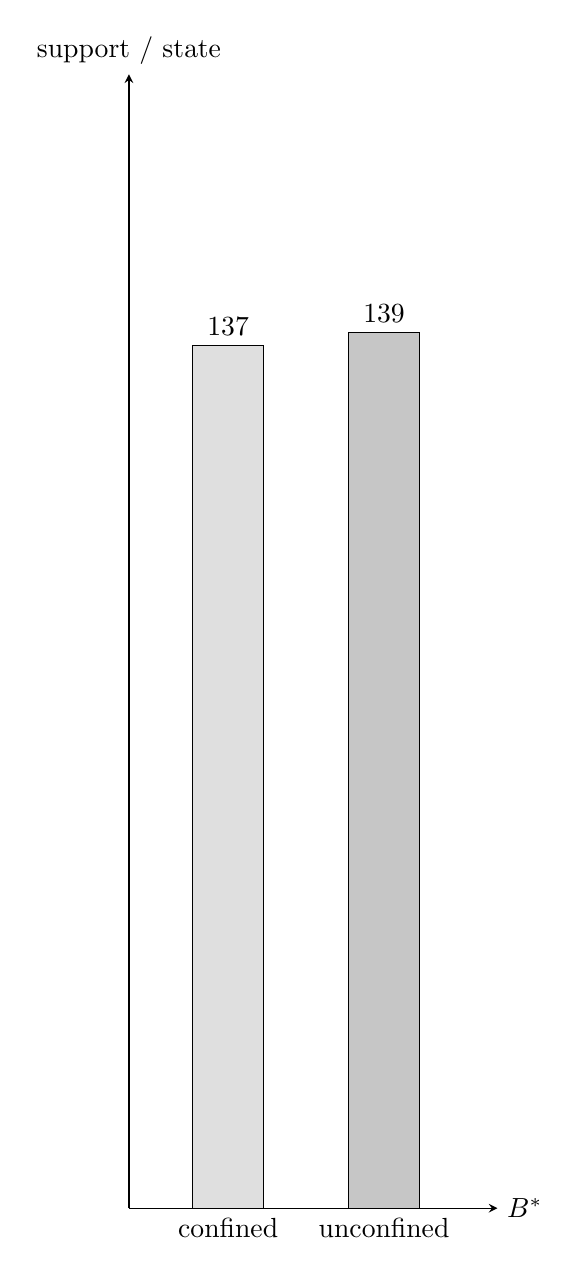
\begin{tikzpicture}[x=1.8cm,y=0.08cm,>=stealth]
\draw[->] (0,0) -- (2.6,0) node[right] {$B^*$};
\draw[->] (0,0) -- (0,180) node[above] {support / state};
\filldraw[fill=gray!25] (0.45,0) rectangle (0.95,137);
\filldraw[fill=gray!45] (1.55,0) rectangle (2.05,139);
\node[below] at (0.7,0) {confined};
\node[below] at (1.8,0) {unconfined};
\node[above] at (0.7,137) {$137$};
\node[above] at (1.8,139) {$139$};
\end{tikzpicture}
\end{center}
\paragraph{Hook / Evidence.} Use the cited confinement, proximity, and transmutation hooks.

\subsection{C6 -- Galactic orbital native window}\label{app:c6}
\paragraph{Native question.} Does the cited long-window galactic trace carry the predicted support mass, residual burden, cadence witness, drift witness, and effective progress-rate profile?
\paragraph{Native readout.}
\begin{itemize}
\item cited galactic window $\omega_{\mathrm{gal}}$
\item structural key \texttt{tetron:4:4:8}
\item frame count / $T_{\mathrm{eval}}=5000$ bip
\item weighting policy $w(\kappa)\equiv 1$
\item native radial grid
\end{itemize}
\paragraph{Native operator chain.}
\[
b(\kappa)\to H_B\to B^*\to \Lambda_b\to R_{\mathrm{rest}}\to \text{cadence witness},\ \text{drift witness},\ v(\omega).
\]
\paragraph{Native output row.}
\begin{center}
\small
\begin{tabular}{lcccccc}
\toprule
Row & Key & $B^*$ & $\Lambda_b$ & $R_{\mathrm{rest}}$ [trit/bip] & Cadence spectrum [cyc/bip] & Drift \\
\midrule
C6.A & tetron:4:4:8 & 137 & 8 & 0.0123 & $\{1/4,3/8\}$ & plateau \\
\bottomrule
\end{tabular}
\end{center}
\paragraph{Temporal Conversion Block.} Temporal conversion is a normal chain-rule expansion on the cited native row. At the current witness radius of $24$ kpc, the available speed witnesses are
\[
v_{\mathrm{classical}}=63.50852961085884\ \text{km/s},\qquad
v_{\mathrm{temporal}}=220.0\ \text{km/s},\qquad
v_{\mathrm{flat}}=220.0\ \text{km/s}.
\]
\paragraph{Native figure witness.}
\begin{center}
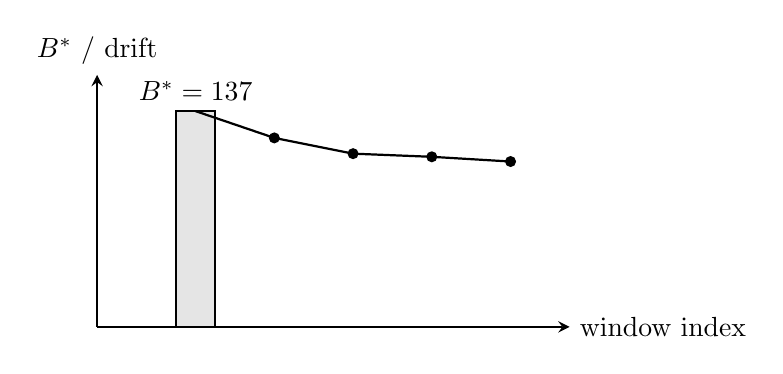
\begin{tikzpicture}[x=1.0cm,y=0.02cm,>=stealth,thick]
\draw[->] (0,0) -- (6,0) node[right] {window index};
\draw[->] (0,0) -- (0,160) node[above] {$B^*$ / drift};
\draw[fill=gray!20] (1,0) rectangle (1.5,137);
\draw (1.25,137)--(2.25,120)--(3.25,110)--(4.25,108)--(5.25,105);
\foreach \x/\y in {2.25/120,3.25/110,4.25/108,5.25/105}{\fill (\x,\y) circle (2pt);} 
\node[above] at (1.25,137) {$B^*=137$};
\end{tikzpicture}
\end{center}
\paragraph{Hook / Evidence.} Use the cited long-window drift and support hooks.


\subsection{C7 -- Brownian bacteria motion}\label{app:c7}
\paragraph{Native question.} Does the cited recurrent jitter window show the predicted dwell distribution, residual-duration support, cadence-noise band, and service-burden profile?
\paragraph{Native readout.}
\begin{itemize}
\item cited window $\omega_{\mathrm{jit}}$
\item structural key \texttt{tetron:2:2:4}
\item frame count / $T_{\mathrm{eval}}=1024$ bip
\item weighting policy $w(\kappa)\equiv 1$
\item jitter/dwell samples
\end{itemize}
\paragraph{Native operator chain.}
\[
e_\alpha,\ e_\Omega,\ f
\;\to\;
b(\kappa)
\;\to\;
H_B
\;\to\;
B^*
\;\to\;
\Lambda_b
\;\to\;
R_{\mathrm{rest}}
\;\to\;
\text{cadence-noise witness},\ \text{drift witness}.
\]
\paragraph{Native output row.}
\begin{center}
\begin{tabularx}{\linewidth}{@{}lXcclll@{}}
\toprule
Row & Structural key & $B^*$ & $\Lambda_b$ & Dwell distribution & Cadence-noise & Drift \\
\midrule
C7.A & \texttt{tetron:2:2:4} & 2 & 11 & recurrent jitter & jitter band & recurrent \\
\bottomrule
\end{tabularx}
\end{center}
\paragraph{Temporal Conversion Block.} Temporal conversion is a normal chain-rule expansion on the cited native row. This test is retained in native units.
\paragraph{Native figure witness.}
\begin{center}
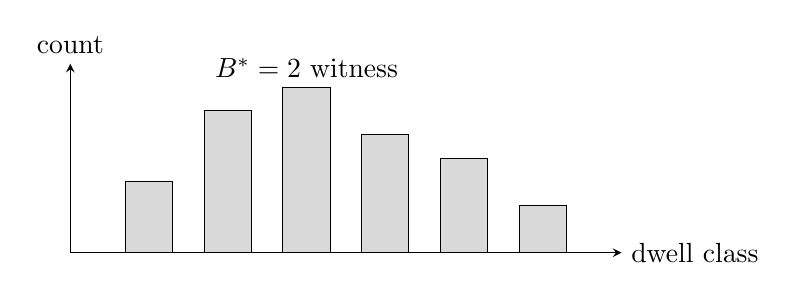
\begin{tikzpicture}[x=1.0cm,y=0.3cm,>=stealth]
\draw[->] (0,0) -- (7,0) node[right] {dwell class};
\draw[->] (0,0) -- (0,8) node[above] {count};
\foreach \x/\h in {1/3,2/6,3/7,4/5,5/4,6/2}{\filldraw[fill=gray!30] (\x-0.3,0) rectangle (\x+0.3,\h);} 
\node[above] at (3,7) {$B^*=2$ witness};
\end{tikzpicture}
\end{center}
\paragraph{Hook / Evidence.} Use the cited recurrent-jitter and dwell-distribution hooks.

